%%%%%%%%%%%%%%%%%%%%%%%%%%%%
% A minimalistic template  %
% for proposal submission  %
% to HKRGC GRF             %
% Use at your own risk!    %
% By Zhiya Zuo             %
%    zhiyazuo@icloud.com   %
%    August-20 2020        %
%%%%%%%%%%%%%%%%%%%%%%%%%%%%

\documentclass[12pt,notitlepage]{article}
%\documentclass[12pt]{apa6}
%\usepackage[utf8]{inputenc}
%%%%%%%%%%%%%%%%%%%%%%%%%
\usepackage{fontspec}
\setmainfont{Times New Roman}
%%%%%%%%%%%%%%%%%%%%%%%%%
\usepackage[a4paper,margin=2.5cm]{geometry}
%\geometry{margin=2.5cm, a4paper}
%%%%%%%%%%%%%%%%%%%%%%%%%
\usepackage{setspace}
\singlespacing
%%%%%%%%%%%%%%%%%%%%%%%%%
\usepackage{minted}
%%%%%%%%%%%%%%%%%%%%%%%%%
\usepackage{titling}
\pretitle{\vskip -5ex\begin{center}\normalfont\bfseries}
%\posttitle{\vskip 0pt}
\posttitle{\end{center}\vskip -5ex}
\preauthor{}
\postauthor{}
\predate{}
\postdate{}
%%%%%%%%%%%%%%%%%%%%%%%%%
\author{}
\title{\vskip -10ex Background of Research}
\date{}
%%%%%%%%%%%%%%%%%%%%%%%%%
\usepackage{titlesec}
\titlespacing{\title}{0pt}{0.2ex}{0ex}
\titleformat{\title}
{\centering\normalfont\bfseries}
{}{0pt}{}
%
\titlespacing{\section}{0pt}{0.2ex}{0ex}
\titleformat{\section}
{\centering\normalfont\bfseries}
{}{0pt}{}
%
\titlespacing{\subsection}{0pt}{0.2ex}{0ex}
\titleformat{\subsection}
{\normalfont\bfseries\itshape}
{}{0pt}{}
%%%%%%%%%%%%%%%%%%%%%%%%%
\usepackage{lipsum}
%%%%%%%%%%%%%%%%%%%%%%%%%
\usepackage{float}
\usepackage{graphicx}
\usepackage{amsmath}
\usepackage{hyperref}
\usepackage[capitalise,noabbrev]{cleveref}
%%%%%%%%%%%%%%%%%%%%%%%%%
%\pagenumbering{gobble}
%%%%%%%%%%%%%%%%%%%%%%%%%
\usepackage{csquotes}
%%%%%%%%%%%%%%%%%%%%%%%%%
\usepackage[american]{babel}
\usepackage[sortcites=true,sorting=nyt,style=apa,doi=false,isbn=false,eprint=false]{biblatex}
\DeclareLanguageMapping{american}{american-apa}
\DeclareDelimFormat[textcite]{finalnamedelim}{%
  \ifnumgreater{\value{liststop}}{2}{\finalandcomma}{}%
  \addspace\bibstring{and}\space}
%\DeclareDelimFormat[parencite]{finalnamedelim}{\addspace\&\space}
\addbibresource{references.bib}
%%%%%%%%%%%%%%%%%%%%%%%%%

\begin{document}

\maketitle

\section{Introduction}
\lipsum[1-2]

The titling package~\parencite{titling} provides control over the typesetting of the \mintinline{TeX}{\maketitle} and \mintinline{TeX}{\thanks} commands.
The values of \mintinline{TeX}{\title}, \mintinline{TeX}{\author} and \mintinline{TeX}{\date} are also retained,
and there may be multiple titles in a document.
New titling elements may be defined for printing by \mintinline{TeX}{\maketitle}.

\section{Theories}
\lipsum[4-5]

\section{Hypothesis Development}
\lipsum[6-7]

\section{Research plan and methodology}
%\lipsum[8]
Our College of Business (CB) is located in the tower of
the distinctive Lau Ming Wai Academic Building (LAU, \cref{fig:ac3}),
at our City University of Hong Kong (CityU) campus,
which is situated in the conveniently prime location of Kowloon Tong.
As CityU flourishes, we have created a beautiful space that is highly conducive to learning and teaching.

\subsection{Data Collection}
\lipsum[9-10]

Finally let's show some example tables~\cref{tab:1}.

\subsection{Analysis}
The following introduces the name of Hong Kong~\parencite[\cref{fig:hk};][]{wiki:hk}.
The name of the territory, first romanised as ``He-Ong-Kong'' in 1780,
originally referred to a small inlet located between Aberdeen Island and the southern coast of Hong Kong Island. Aberdeen was an initial point of contact between British sailors and local fishermen.
Although the source of the romanised name is unknown,
it is generally believed to be an early phonetic rendering of the Cantonese pronunciation hēung góng. The name translates as ``fragrant harbour'' or ``incense harbour''.
``Fragrant'' may refer to the sweet taste of the harbour's freshwater influx from the Pearl River or
to the odour from incense factories lining the coast of northern Kowloon.
The incense was stored near Aberdeen Harbour for export before Victoria Harbour developed.
Sir John Davis (the second colonial governor) offered an alternative origin;
Davis said that the name derived from ``Hoong-keang'' (``red torrent''),
reflecting the colour of soil over which a waterfall on the island flowed.
The simplified name Hong Kong was frequently used by 1810.
The name was also commonly written as the single word Hongkong until 1926, when the government officially adopted the two-word name.
Some corporations founded during the early colonial era still keep this name, including Hongkong Land, Hongkong Electric Company, Hongkong and Shanghai Hotels and the Hongkong and Shanghai Banking Corporation (HSBC).
%%%%%%%%%%%% END MAIN TEXT %%%%%%%%%%%%
%%%%%%%%%%%% fig and tab %%%%%%%%%%%%
\clearpage
\pagenumbering{arabic}
\setcounter{page}{1}
\section{Figures}

\begin{figure}[H]
  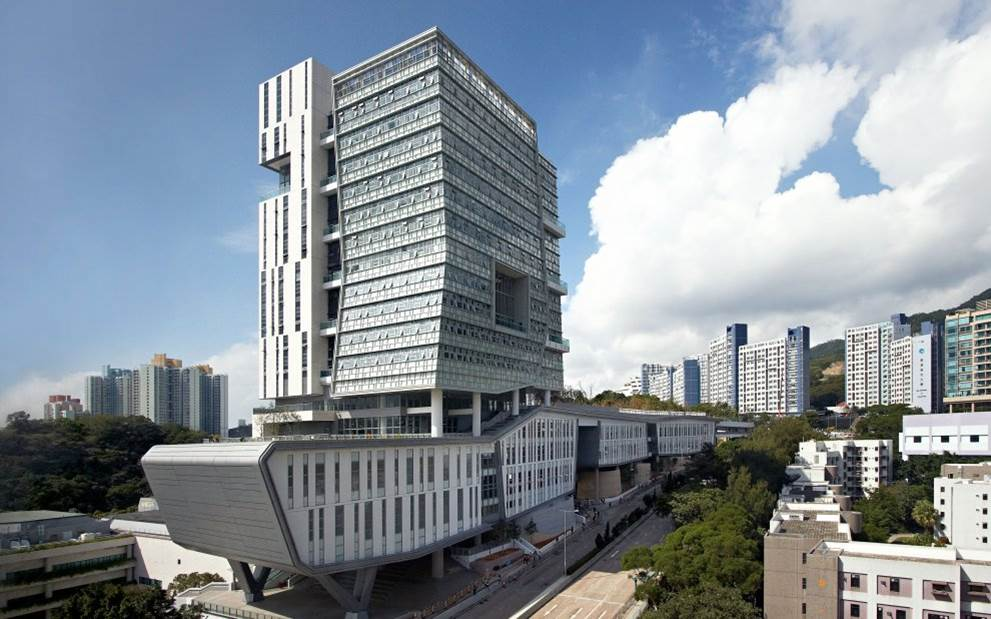
\includegraphics[width=\linewidth]{AC3}
  \caption{Lau Ming Wai Academic Building (LAU). Image source: \url{https://www.cb.cityu.edu.hk/exchange/team/}.}
  \label{fig:ac3}
\end{figure}

%\hfill

\begin{figure}[H]
  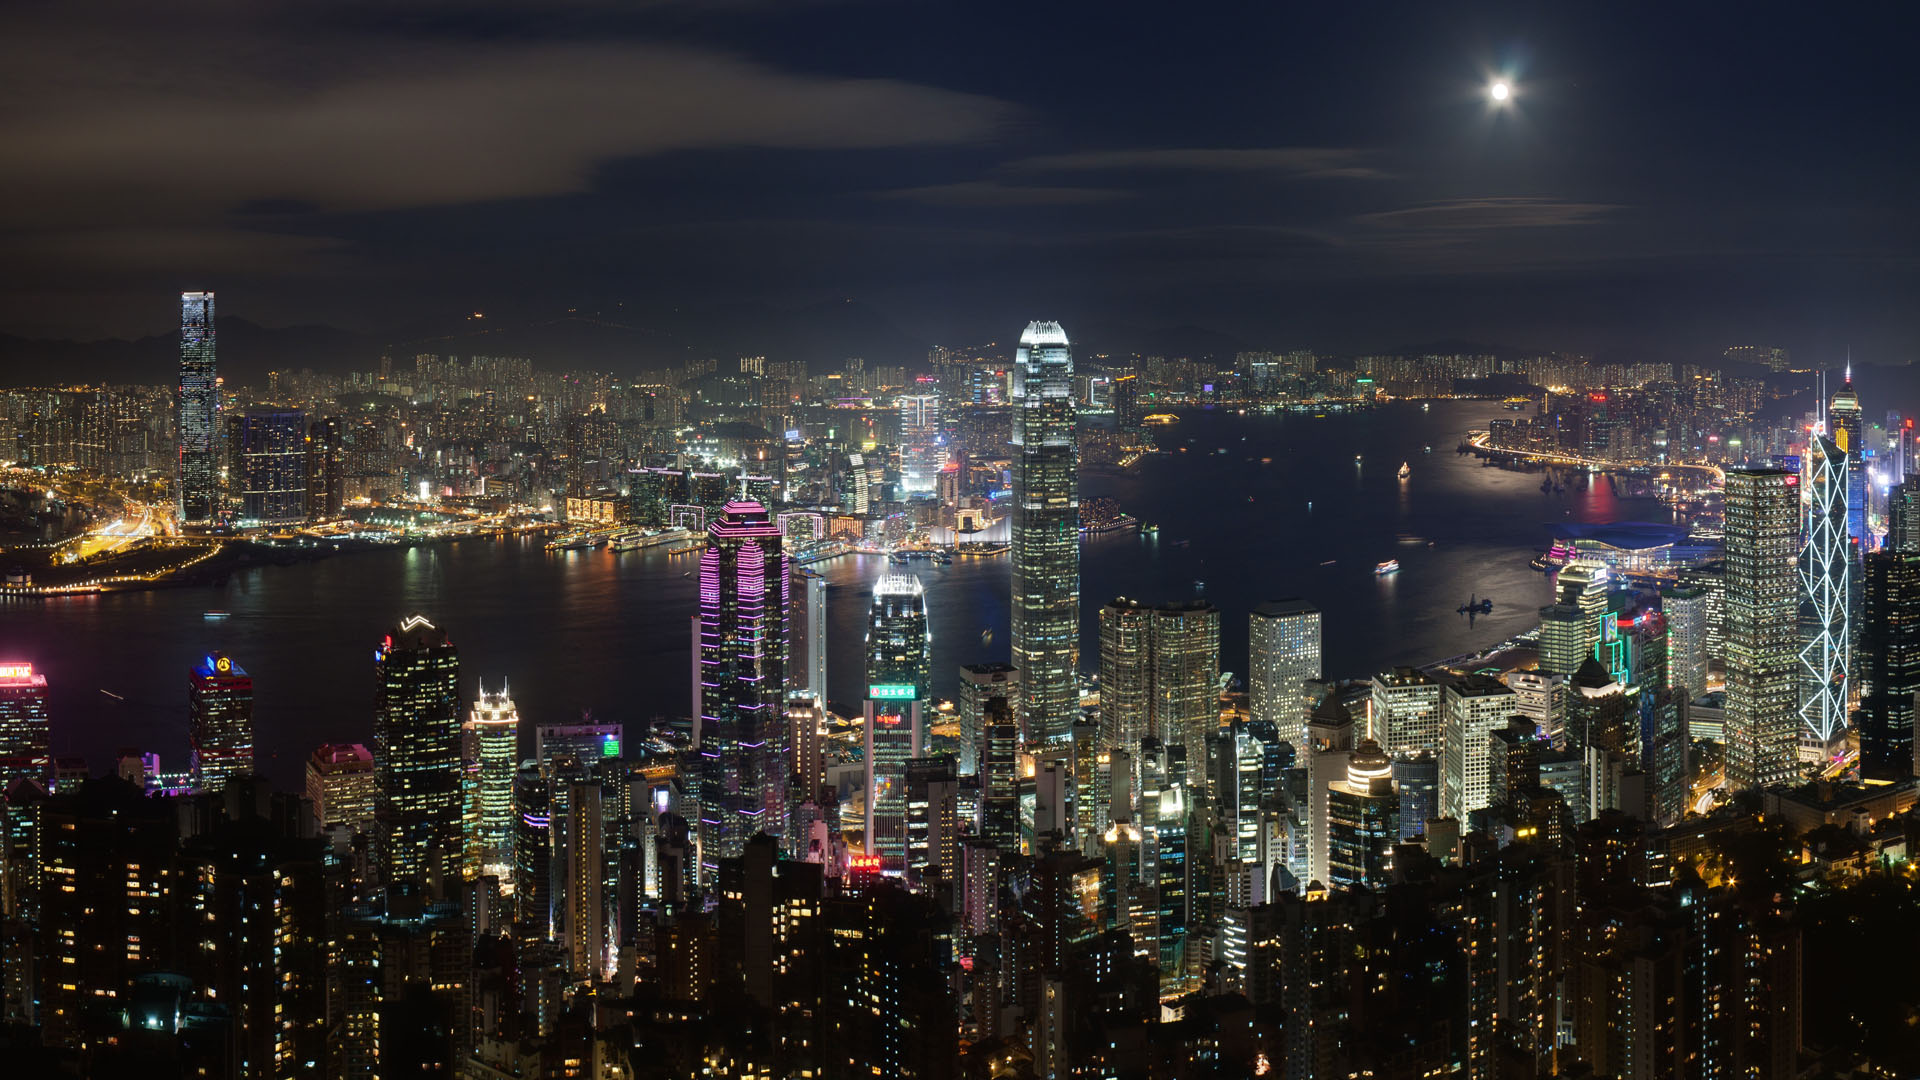
\includegraphics[width=\linewidth]{hk}
  \caption{Hong Kong night view. Image source: \url{https://commons.wikimedia.org/wiki/File:Hong_Kong_Night_view.jpg}}
  \label{fig:hk}
\end{figure}

\section{Tables}
\begin{table}[H]
\centering
\caption{A random table from \url{https://www.overleaf.com/learn/latex/tables}}
\label{tab:1}
\begin{tabular}{ |p{3cm}||p{3cm}|p{3cm}|p{3cm}|  }
 \hline
 \multicolumn{4}{|c|}{Country List} \\
 \hline
 Country Name     or Area Name& ISO ALPHA 2 Code &ISO ALPHA 3 Code&ISO numeric Code\\
 \hline
 Afghanistan   & AF    &AFG&   004\\
 Aland Islands&   AX  & ALA   &248\\
 Albania &AL & ALB&  008\\
 Algeria    &DZ & DZA&  012\\
 American Samoa&   AS  & ASM&016\\
 Andorra& AD  & AND   &020\\
 Angola& AO  & AGO&024\\
 \hline
\end{tabular}
\end{table}

%%%%%%%%%%%% REFERENCES %%%%%%%%%%%%
\clearpage
\pagenumbering{arabic}
\setcounter{page}{1}
\section{References}
\printbibliography[heading=none]

\end{document}
